% Options for packages loaded elsewhere
\PassOptionsToPackage{unicode}{hyperref}
\PassOptionsToPackage{hyphens}{url}
%
\documentclass[
]{book}
\usepackage{lmodern}
\usepackage{amssymb,amsmath}
\usepackage{ifxetex,ifluatex}
\ifnum 0\ifxetex 1\fi\ifluatex 1\fi=0 % if pdftex
  \usepackage[T1]{fontenc}
  \usepackage[utf8]{inputenc}
  \usepackage{textcomp} % provide euro and other symbols
\else % if luatex or xetex
  \usepackage{unicode-math}
  \defaultfontfeatures{Scale=MatchLowercase}
  \defaultfontfeatures[\rmfamily]{Ligatures=TeX,Scale=1}
\fi
% Use upquote if available, for straight quotes in verbatim environments
\IfFileExists{upquote.sty}{\usepackage{upquote}}{}
\IfFileExists{microtype.sty}{% use microtype if available
  \usepackage[]{microtype}
  \UseMicrotypeSet[protrusion]{basicmath} % disable protrusion for tt fonts
}{}
\makeatletter
\@ifundefined{KOMAClassName}{% if non-KOMA class
  \IfFileExists{parskip.sty}{%
    \usepackage{parskip}
  }{% else
    \setlength{\parindent}{0pt}
    \setlength{\parskip}{6pt plus 2pt minus 1pt}}
}{% if KOMA class
  \KOMAoptions{parskip=half}}
\makeatother
\usepackage{xcolor}
\IfFileExists{xurl.sty}{\usepackage{xurl}}{} % add URL line breaks if available
\IfFileExists{bookmark.sty}{\usepackage{bookmark}}{\usepackage{hyperref}}
\hypersetup{
  pdftitle={GEE学習サイト},
  pdfauthor={Tamaki.M},
  hidelinks,
  pdfcreator={LaTeX via pandoc}}
\urlstyle{same} % disable monospaced font for URLs
\usepackage{longtable,booktabs}
% Correct order of tables after \paragraph or \subparagraph
\usepackage{etoolbox}
\makeatletter
\patchcmd\longtable{\par}{\if@noskipsec\mbox{}\fi\par}{}{}
\makeatother
% Allow footnotes in longtable head/foot
\IfFileExists{footnotehyper.sty}{\usepackage{footnotehyper}}{\usepackage{footnote}}
\makesavenoteenv{longtable}
\usepackage{graphicx,grffile}
\makeatletter
\def\maxwidth{\ifdim\Gin@nat@width>\linewidth\linewidth\else\Gin@nat@width\fi}
\def\maxheight{\ifdim\Gin@nat@height>\textheight\textheight\else\Gin@nat@height\fi}
\makeatother
% Scale images if necessary, so that they will not overflow the page
% margins by default, and it is still possible to overwrite the defaults
% using explicit options in \includegraphics[width, height, ...]{}
\setkeys{Gin}{width=\maxwidth,height=\maxheight,keepaspectratio}
% Set default figure placement to htbp
\makeatletter
\def\fps@figure{htbp}
\makeatother
\setlength{\emergencystretch}{3em} % prevent overfull lines
\providecommand{\tightlist}{%
  \setlength{\itemsep}{0pt}\setlength{\parskip}{0pt}}
\setcounter{secnumdepth}{5}
\usepackage{booktabs}
\usepackage[]{natbib}
\bibliographystyle{apalike}

\title{GEE学習サイト}
\author{Tamaki.M}
\date{2020-12-07}

\begin{document}
\maketitle

{
\setcounter{tocdepth}{1}
\tableofcontents
}
\hypertarget{ux521dux3081ux306b}{%
\chapter*{初めに}\label{ux521dux3081ux306b}}
\addcontentsline{toc}{chapter}{初めに}

このサイトでは、Google earth engineを活用して洪水被害図を作成する方法について詳細に紹介しています。UN Spiderが提供しているコードにのっとって説明をしています。元のサイトを確認したい方は、以下のURLから飛ぶことができます。
(\url{https://un-spider.org/advisory-support/recommended-practices/recommended-practice-google-earth-engine-flood-mapping/step-by-step})

コードを詳しく知る前に、まずはどのようなものが出来上がるのか確認したいという方は、以下のサイトに従って作成してみてください。
(\url{https://tamak1313.github.io/cosmobook/})

\hypertarget{ux5bfeux8c61ux8005}{%
\section{対象者}\label{ux5bfeux8c61ux8005}}

\begin{itemize}
\item
  衛星データ初心者
\item
  GEE初心者
\end{itemize}

\hypertarget{ux4f5cux696dux74b0ux5883}{%
\section{作業環境}\label{ux4f5cux696dux74b0ux5883}}

2020年12月現在
Windows 10 64bit

\hypertarget{section}{%
\chapter{1}\label{section}}

まずは以下のコードを自分の研究対象に書き換えてみましょう。
(\url{https://un-spider.org/advisory-support/recommended-practices/recommended-practice-google-earth-engine-flood-mapping/step-by-step})

対象エリア、期間は以下の方法で変更することができます。

\hypertarget{ux5bfeux8c61ux30a8ux30eaux30a2}{%
\section{対象エリア}\label{ux5bfeux8c61ux30a8ux30eaux30a2}}

①地図上のツールバーの一番右(■)をクリックする。研究対象エリアを四角形で囲むことができる。

\begin{figure}
\centering
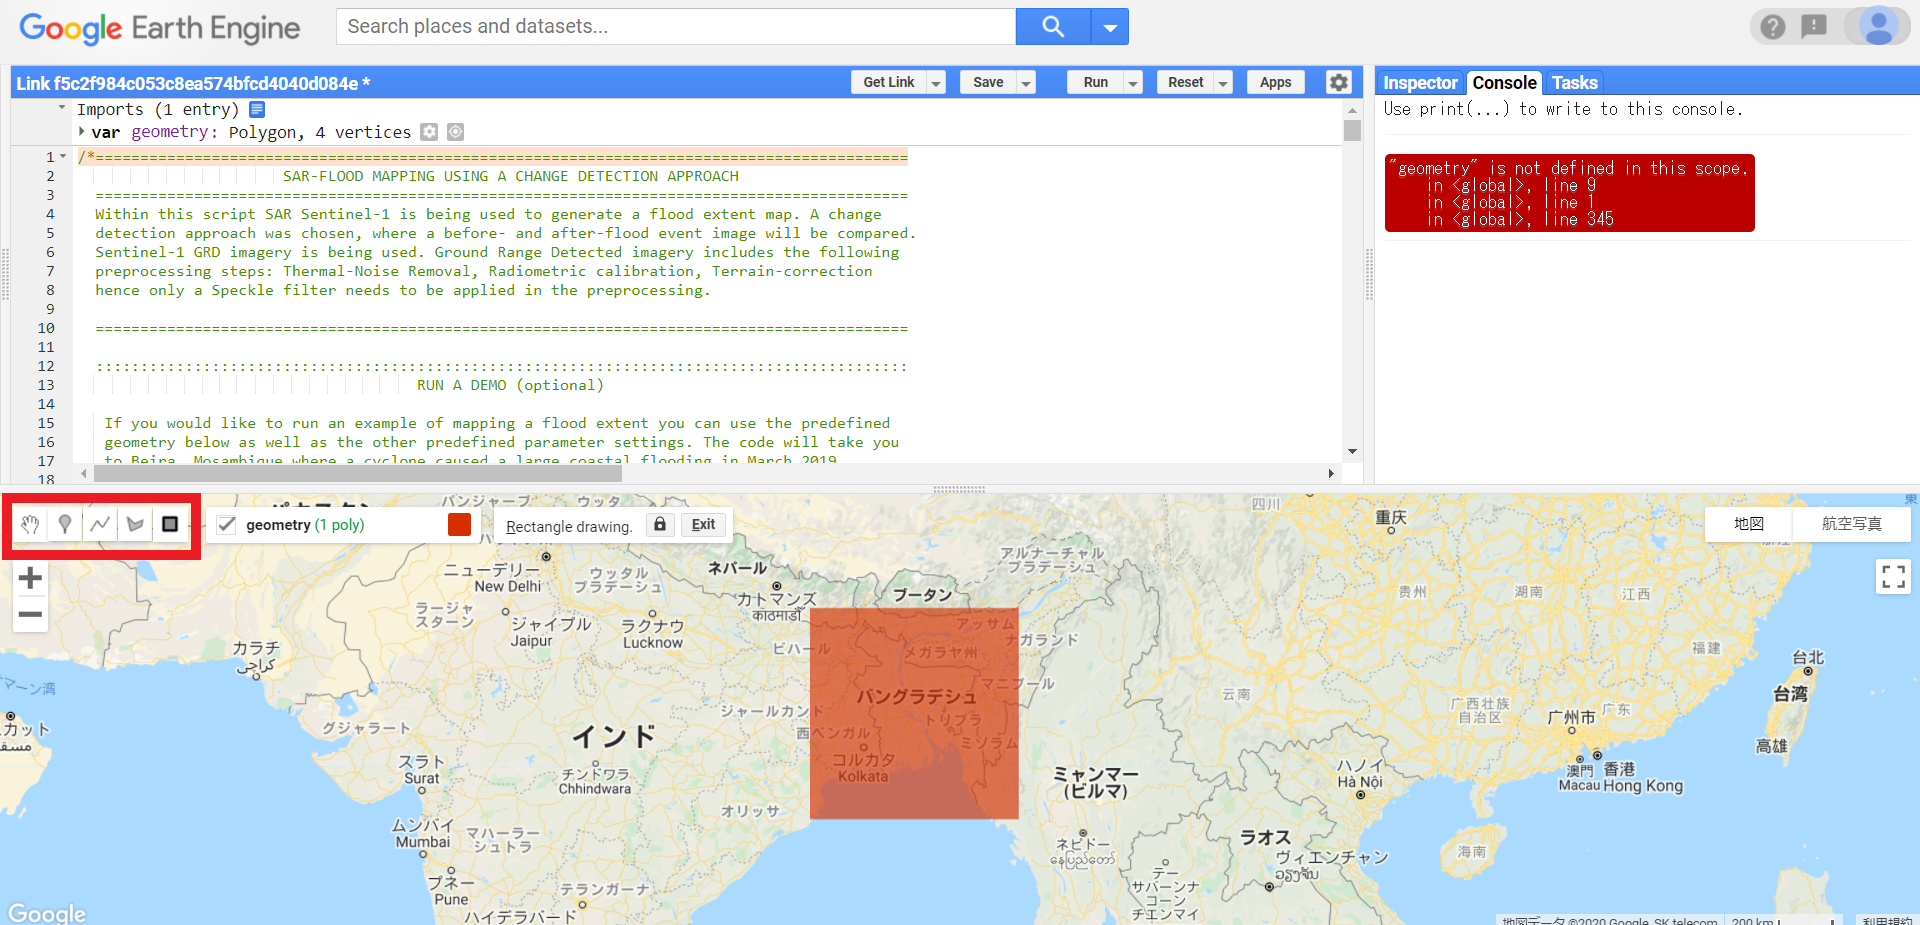
\includegraphics{images/geepolygon1.png}
\caption{GEE polygon1}
\end{figure}

②地図上のツールバーの右から2番目(5角形)をクリックする。研究対象エリアにピンを立て、必要最低限のエリアを選択することが可能。  

\begin{figure}
\centering
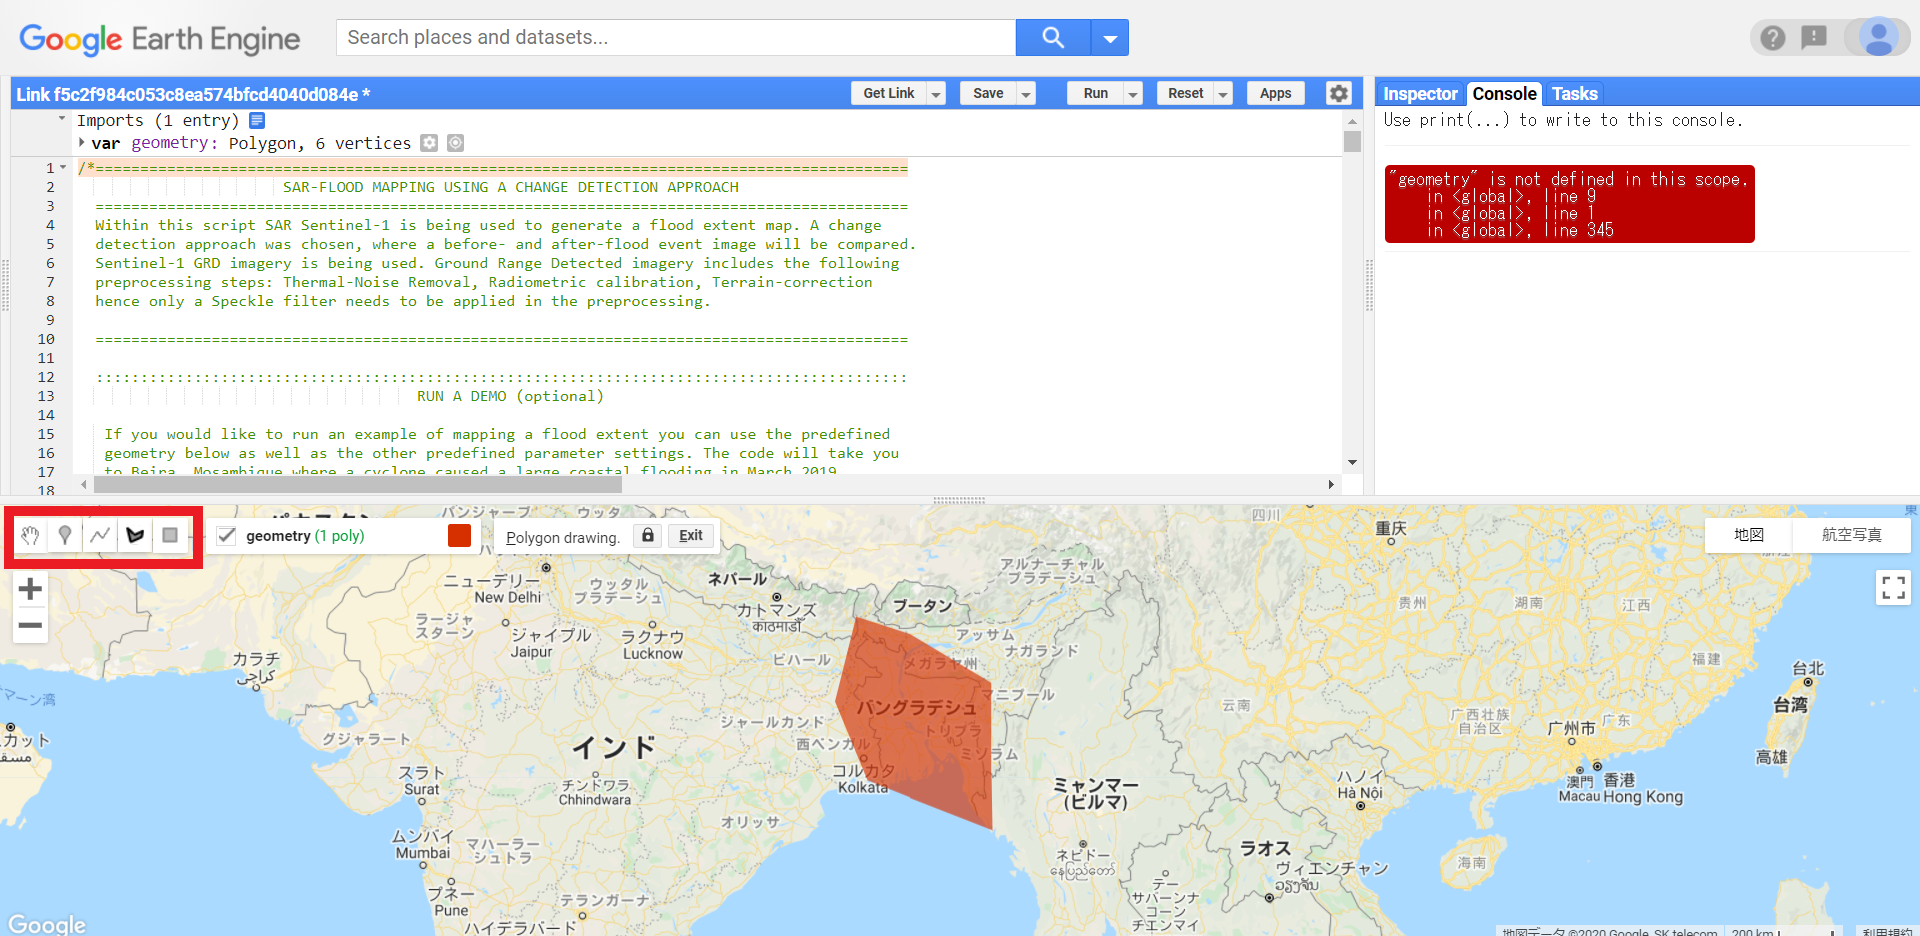
\includegraphics{images/geepolygon2.png}
\caption{GEE polygon2}
\end{figure}

\hypertarget{ux5bfeux8c61ux671fux9593}{%
\section{対象期間}\label{ux5bfeux8c61ux671fux9593}}

洪水前後の日時(期間)を設定する。  

*使用するデータはSentinel-1で6日周期であることに留意。

\hypertarget{ux5404ux7a2eux8a2dux5b9a}{%
\section{各種設定}\label{ux5404ux7a2eux8a2dux5b9a}}

\hypertarget{ux30c7ux30fcux30bfux306eux9078ux629eux3068ux524dux51e6ux7406}{%
\chapter{データの選択と前処理}\label{ux30c7ux30fcux30bfux306eux9078ux629eux3068ux524dux51e6ux7406}}

用語集
+ ジオメトリー(geometry):

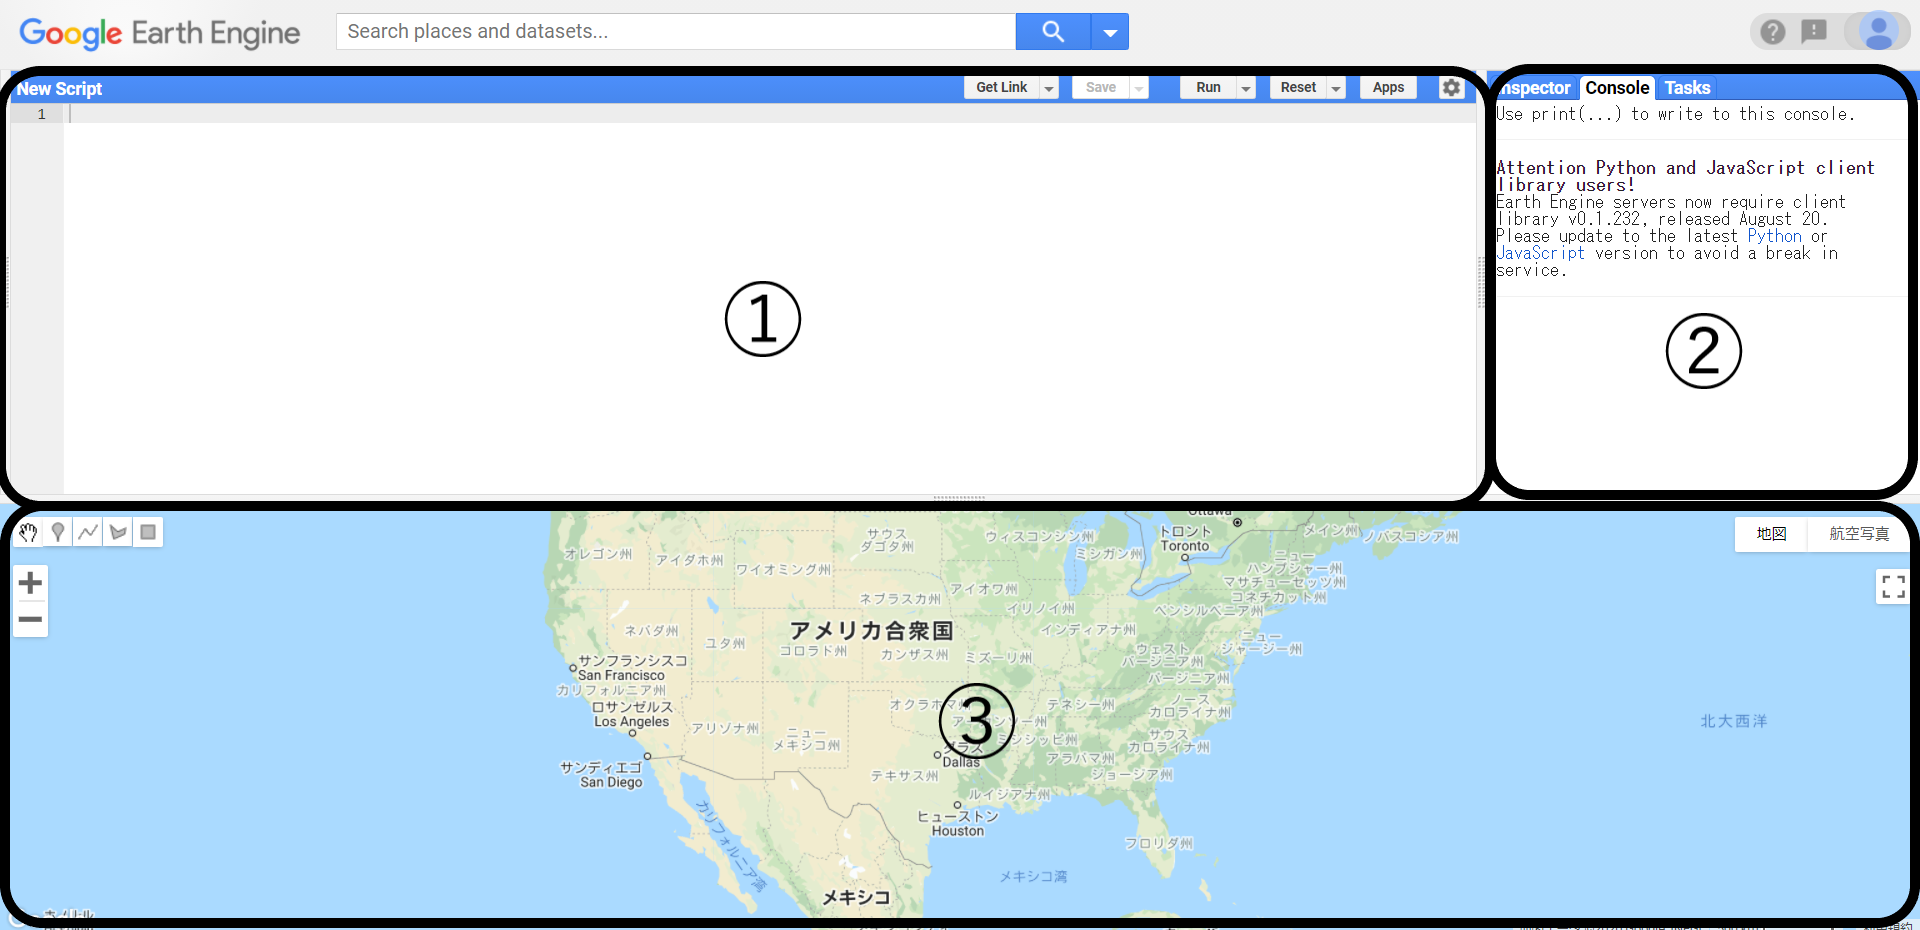
\includegraphics{images/GEE.png}
①

②

③

\begin{verbatim}
var aoi = ee.FeatureCollection(geometry);    //ジオメトリーの名称を変更する 

// パラメーターを定義する前のSentinel-1 GRD(対象データ)をロードし、フィルターをかける 
var collection= ee.ImageCollection('COPERNICUS/S1_GRD')
  .filter(ee.Filter.eq('instrumentMode','IW'))
  .filter(ee.Filter.listContains('transmitterReceiverPolarisation', polarization))
  .filter(ee.Filter.eq('orbitProperties_pass',pass_direction)) 
  .filter(ee.Filter.eq('resolution_meters',10))
  //.filter(ee.Filter.eq('relativeOrbitNumber_start',relative_orbit ))
  .filterBounds(aoi)
  .select(polarization);
  
// Select images by predefined dates
var before_collection = collection.filterDate(before_start, before_end);
var after_collection = collection.filterDate(after_start,after_end);

// Print selected tiles to the console

      // メタデータからデータを抽出する(メタデータ::主となるデータの説明書きが書いてあるデータ)
      function dates(imgcol){
        var range = imgcol.reduceColumns(ee.Reducer.minMax(), ["system:time_start"]);
        var printed = ee.String('from ')
          .cat(ee.Date(range.get('min')).format('YYYY-MM-dd'))
          .cat(' to ')
          .cat(ee.Date(range.get('max')).format('YYYY-MM-dd'));
        return printed;
      }
      // コンソールに洪水前画像を表示する
      var before_count = before_collection.size();
      print(ee.String('Tiles selected: Before Flood ').cat('(').cat(before_count).cat(')'),
        dates(before_collection), before_collection);
      
      // コンソールに洪水後画像を表示する
      var after_count = before_collection.size();
      print(ee.String('Tiles selected: After Flood ').cat('(').cat(after_count).cat(')'),
        dates(after_collection), after_collection);

// 選択したタイルにモザイクをかけ、対象エリアをクリップする
var before = before_collection.mosaic().clip(aoi);
var after = after_collection.mosaic().clip(aoi);

// レーダーの反転をSmoothingすることによって減らす  
var smoothing_radius = 50;
var before_filtered = before.focal_mean(smoothing_radius, 'circle', 'meters');
var after_filtered = after.focal_mean(smoothing_radius, 'circle', 'meters');

\end{verbatim}

\hypertarget{ux6d78ux6c34ux7bc4ux56f2ux306eux7b97ux51fa}{%
\chapter{浸水範囲の算出}\label{ux6d78ux6c34ux7bc4ux56f2ux306eux7b97ux51fa}}

\begin{verbatim}
// 洪水前後画像を計算する
var difference = after_filtered.divide(before_filtered);

// 定義済みの差分しきい値を適用して、洪水範囲マスクを作成 
var threshold = difference_threshold;
var difference_binary = difference.gt(threshold);

//追加的なデータセットを使って、結果を再定義する
      
      // JRCレイヤーInclude JRC layer on surface water seasonality to mask flood pixels from areas
      // of "permanent" water (where there is water > 10 months of the year)
      var swater = ee.Image('JRC/GSW1_0/GlobalSurfaceWater').select('seasonality');
      var swater_mask = swater.gte(10).updateMask(swater.gte(10));
      
      //Flooded layer where perennial water bodies (water > 10 mo/yr) is assigned a 0 value
      var flooded_mask = difference_binary.where(swater_mask,0);
      // final flooded area without pixels in perennial waterbodies
      var flooded = flooded_mask.updateMask(flooded_mask);
      
      // Compute connectivity of pixels to eliminate those connected to 8 or fewer neighbours
      // This operation reduces noise of the flood extent product 
      var connections = flooded.connectedPixelCount();    
      var flooded = flooded.updateMask(connections.gte(8));
      
      // Mask out areas with more than 5 percent slope using a Digital Elevation Model 
      var DEM = ee.Image('WWF/HydroSHEDS/03VFDEM');
      var terrain = ee.Algorithms.Terrain(DEM);
      var slope = terrain.select('slope');
      var flooded = flooded.updateMask(slope.lt(5));

//洪水面積を計算する
// それぞれのピクセルの地域情報を含んだラスターレイヤーを作成 
var flood_pixelarea = flooded.select(polarization)
  .multiply(ee.Image.pixelArea());

// 洪水被害を受けたピクセルの面積を集積
// 演算時間を減らすためのデフォルト設定(正確な結果を算出したい場合は、”bestEffort”をfalseに設定し、maxPixelsを増加させる)
var flood_stats = flood_pixelarea.reduceRegion({
  reducer: ee.Reducer.sum(),              
  geometry: aoi,
  scale: 10, // native resolution 
  //maxPixels: 1e9,
  bestEffort: true
  });

// メートルをヘクタールに変換  
var flood_area_ha = flood_stats
  .getNumber(polarization)
  .divide(10000)
  .round(); 
\end{verbatim}

\hypertarget{ux88abux5bb3ux8a55ux4fa1}{%
\chapter{被害評価}\label{ux88abux5bb3ux8a55ux4fa1}}

\hypertarget{estimated-number-of-exposed-people}{%
\section{``Estimated number of exposed people''}\label{estimated-number-of-exposed-people}}

\begin{verbatim}
// JRCレイヤー(JRC Global Human Settlement Popluation Density layer)をロードする
// Resolution: 250. 1セル当たりの人口
var population_count = ee.Image('JRC/GHSL/P2016/POP_GPW_GLOBE_V1/2015').clip(aoi);
\end{verbatim}

\hypertarget{ux88abux5bb3ux4ebaux53e3ux3092ux7b97ux51faux3059ux308b}{%
\subsection{被害人口を算出する}\label{ux88abux5bb3ux4ebaux53e3ux3092ux7b97ux51faux3059ux308b}}

\begin{verbatim}
// GHSL(the Global Human Settlement Layer))を投影させる
var GHSLprojection = population_count.projection();

// GHSLスケールに洪水レイヤーをReprojectする?
var flooded_res1 = flooded
    .reproject({
    crs: GHSLprojection
  });

// the resampled flood layerを使い、被害人口を示すレイヤーを作成する
var population_exposed = population_count
  .updateMask(flooded_res1)
  .updateMask(population_count);

//被害人口ラスターのピクセルあたりの数値を計算する 
var stats = population_exposed.reduceRegion({
  reducer: ee.Reducer.sum(),
  geometry: aoi,
  scale: 250,
  maxPixels:1e9 
});

// 被害人口を整数値で算出する
var number_pp_exposed = stats.getNumber('population_count').round();
\end{verbatim}

\hypertarget{estimated-affected-cropland}{%
\section{``Estimated affected cropland''}\label{estimated-affected-cropland}}

\begin{verbatim}
// MODIS Land Cover Type Yearly Global 500mを使用する
// 最新の土地被覆データ(MODIS)をフィルターにかける 
var LC = ee.ImageCollection('MODIS/006/MCD12Q1')
  .filterDate('2014-01-01',after_end)
  .sort('system:index',false)
  .select("LC_Type1")
  .first()
  .clip(aoi);

// the classes cropland (>60%) and Cropland/Natural である耕作地ピクセルだけを抽出する
// 植生モザイク: mosaics of small-scale cultivation 40-60% incl. natural vegetation
var cropmask = LC
  .eq(12)
  .or(LC.eq(14))
var cropland = LC
  .updateMask(cropmask)
  
// MODISを投影させる
var MODISprojection = LC.projection();

// MODISスケールにflood layerをReprojectする
var flooded_res = flooded
    .reproject({
    crs: MODISprojection
  });

// the resampled flood layerを使って、耕作地への影響を算出する
var cropland_affected = flooded_res
  .updateMask(cropland)

// get pixel area of affected cropland layer
var crop_pixelarea = cropland_affected
  .multiply(ee.Image.pixelArea()); //calcuate the area of each pixel 

// affected cropland layerのピクセルを足し合わせる
var crop_stats = crop_pixelarea.reduceRegion({
  reducer: ee.Reducer.sum(), //sum all pixels with area information                
  geometry: aoi,
  scale: 500,
  maxPixels: 1e9
  });
  
// ヘクタールに換算する
var crop_area_ha = crop_stats
  .getNumber(polarization)
  .divide(10000)
  .round();
\end{verbatim}

\hypertarget{estimated-affected-urban-area}{%
\section{``Estimated affected urban area''}\label{estimated-affected-urban-area}}

\begin{verbatim}
// Using the same MODIS Land Cover Product 
// 都市エリアをフィルターにかける
var urbanmask = LC.eq(13)
var urban = LC
  .updateMask(urbanmask)

//Calculate affected urban areas using the resampled flood layer
var urban_affected = urban
  .mask(flooded_res)
  .updateMask(urban);

// get pixel area of affected urban layer
var urban_pixelarea = urban_affected
  .multiply(ee.Image.pixelArea()); //calcuate the area of each pixel 

// sum pixels of affected cropland layer
var urban_stats = urban_pixelarea.reduceRegion({
  reducer: ee.Reducer.sum(), //sum all pixels with area information                
  geometry: aoi,
  scale: 500,
  bestEffort: true,
  });

// convert area to hectares
var urban_area_ha = urban_stats
  .getNumber('LC_Type1')
  .divide(10000)
  .round();
\end{verbatim}

\hypertarget{ux30d7ux30edux30c0ux30afux30c8ux306eux8868ux793a}{%
\chapter{プロダクトの表示}\label{ux30d7ux30edux30c0ux30afux30c8ux306eux8868ux793a}}

We have finished a nice book.

\hypertarget{map-production}{%
\chapter{MAP PRODUCTION}\label{map-production}}

\hypertarget{ux5730ux56f3ux4e0aux306bux7d50ux679cux3092ux8868ux793aux3059ux308bux2460}{%
\section{地図上に結果を表示する①}\label{ux5730ux56f3ux4e0aux306bux7d50ux679cux3092ux8868ux793aux3059ux308bux2460}}

\begin{figure}
\centering
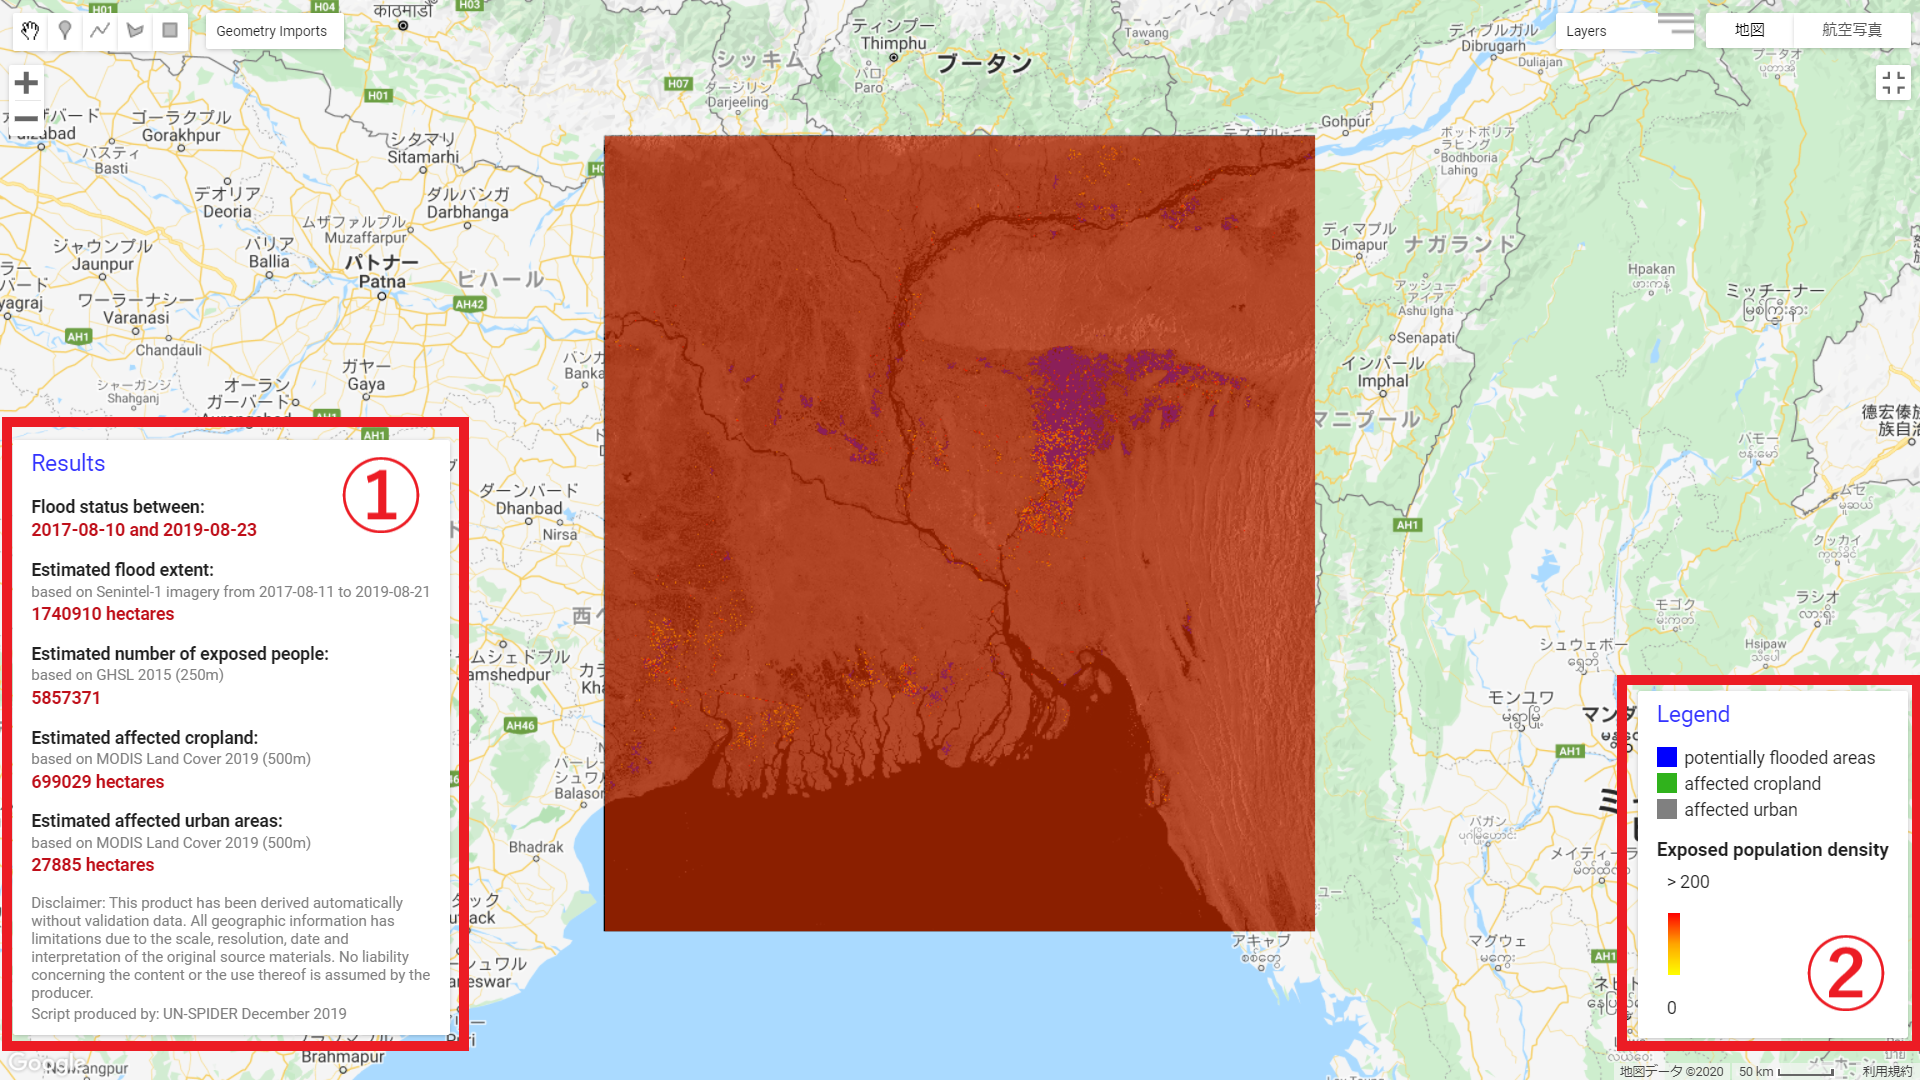
\includegraphics{images/example1.png}
\caption{パネル表示①}
\end{figure}

\hypertarget{ux7d50ux679cux304cux8868ux793aux3055ux308cux308bux30d1ux30cdux30ebux306eux4f4dux7f6eux3092ux8a2dux5b9aux3059ux308b}{%
\subsection{結果が表示されるパネルの位置を設定する  }\label{ux7d50ux679cux304cux8868ux793aux3055ux308cux308bux30d1ux30cdux30ebux306eux4f4dux7f6eux3092ux8a2dux5b9aux3059ux308b}}

\begin{verbatim}
var results = ui.Panel({
  style: {
    position: 'bottom-left',
    padding: '8px 15px',
    width: '350px'
  }
});
\end{verbatim}

\hypertarget{ux8868ux793aux5f62ux5f0fux3092ux8a2dux5b9aux3059ux308b}{%
\subsection{表示形式を設定する}\label{ux8868ux793aux5f62ux5f0fux3092ux8a2dux5b9aux3059ux308b}}

\begin{verbatim}
var textVis = {
  'margin':'0px 8px 2px 0px',
  'fontWeight':'bold'
  };
var numberVIS = {
  'margin':'0px 0px 15px 0px', 
  'color':'bf0f19',
  'fontWeight':'bold'
  };
var subTextVis = {
  'margin':'0px 0px 2px 0px',
  'fontSize':'12px',
  'color':'grey'
  };

var titleTextVis = {
  'margin':'0px 0px 15px 0px',
  'fontSize': '18px', 
  'font-weight':'', 
  'color': '3333ff'
  };
\end{verbatim}

\hypertarget{ux7d50ux679cux306eux30e9ux30d9ux30ebux3092ux4f5cux6210ux3059ux308b}{%
\subsection{結果のラベルを作成する}\label{ux7d50ux679cux306eux30e9ux30d9ux30ebux3092ux4f5cux6210ux3059ux308b}}

\begin{verbatim}
// タイトル
var title = ui.Label('Results', titleTextVis);
// "Flood status between"
var text1 = ui.Label('Flood status between:',textVis);
var number1 = ui.Label(after_start.concat(" and ",after_end),numberVIS);

// "Estimated flood extent"
var text2 = ui.Label('Estimated flood extent:',textVis);
var text2_2 = ui.Label('Please wait...',subTextVis);
dates(after_collection).evaluate(function(val){text2_2.setValue('based on Senintel-1 imagery '+val)});
var number2 = ui.Label('Please wait...',numberVIS); 
flood_area_ha.evaluate(function(val){number2.setValue(val+' hectares')}),numberVIS;

// "Estimated number of exposed people"
var text3 = ui.Label('Estimated number of exposed people: ',textVis);
var text3_2 = ui.Label('based on GHSL 2015 (250m)',subTextVis);
var number3 = ui.Label('Please wait...',numberVIS);
number_pp_exposed.evaluate(function(val){number3.setValue(val)}),numberVIS;

// "Estimated affected cropland"
var MODIS_date = ee.String(LC.get('system:index')).slice(0,4);
var text4 = ui.Label('Estimated affected cropland:',textVis);
var text4_2 = ui.Label('Please wait', subTextVis)
MODIS_date.evaluate(function(val){text4_2.setValue('based on MODIS Land Cover '+val +' (500m)')}), subTextVis;
var number4 = ui.Label('Please wait...',numberVIS);
crop_area_ha.evaluate(function(val){number4.setValue(val+' hectares')}),numberVIS;

// "Estimated affected urban area"
var text5 = ui.Label('Estimated affected urban areas:',textVis);
var text5_2 = ui.Label('Please wait', subTextVis)
MODIS_date.evaluate(function(val){text5_2.setValue('based on MODIS Land Cover '+val +' (500m)')}), subTextVis;
var number5 = ui.Label('Please wait...',numberVIS);
urban_area_ha.evaluate(function(val){number5.setValue(val+' hectares')}),numberVIS;

// 責任・権利利関連
var text6 = ui.Label
('Disclaimer: This product has been derived automatically without validation data. All geographic information has limitations due to the scale, resolution, date and interpretation of the original source materials. No liability concerning the content or the use thereof is assumed by the producer.',subTextVis)

// Produced by...
var text7 = ui.Label('Script produced by: UN-SPIDER December 2019', subTextVis)
\end{verbatim}

\hypertarget{ux30d1ux30cdux30ebux306bux30e9ux30d9ux30ebux3092ux52a0ux3048ux308b}{%
\subsection{パネルにラベルを加える}\label{ux30d1ux30cdux30ebux306bux30e9ux30d9ux30ebux3092ux52a0ux3048ux308b}}

\begin{verbatim}
results.add(ui.Panel([
        title,
        text1,
        number1,
        text2,
        text2_2,
        number2,
        text3,
        text3_2,
        number3,
        text4,
        text4_2,
        number4,
        text5,
        text5_2,
        number5,
        text6,
        text7]
      ));

// 地図にパネルを加える 
Map.add(results);
\end{verbatim}

\hypertarget{ux51e1ux4f8bux3092ux4f5cux6210ux3059ux308bux2461}{%
\section{凡例を作成する②}\label{ux51e1ux4f8bux3092ux4f5cux6210ux3059ux308bux2461}}

(参考:\url{https://mygeoblog.com/2016/12/09/add-a-legend-to-to-your-gee-map/})\\
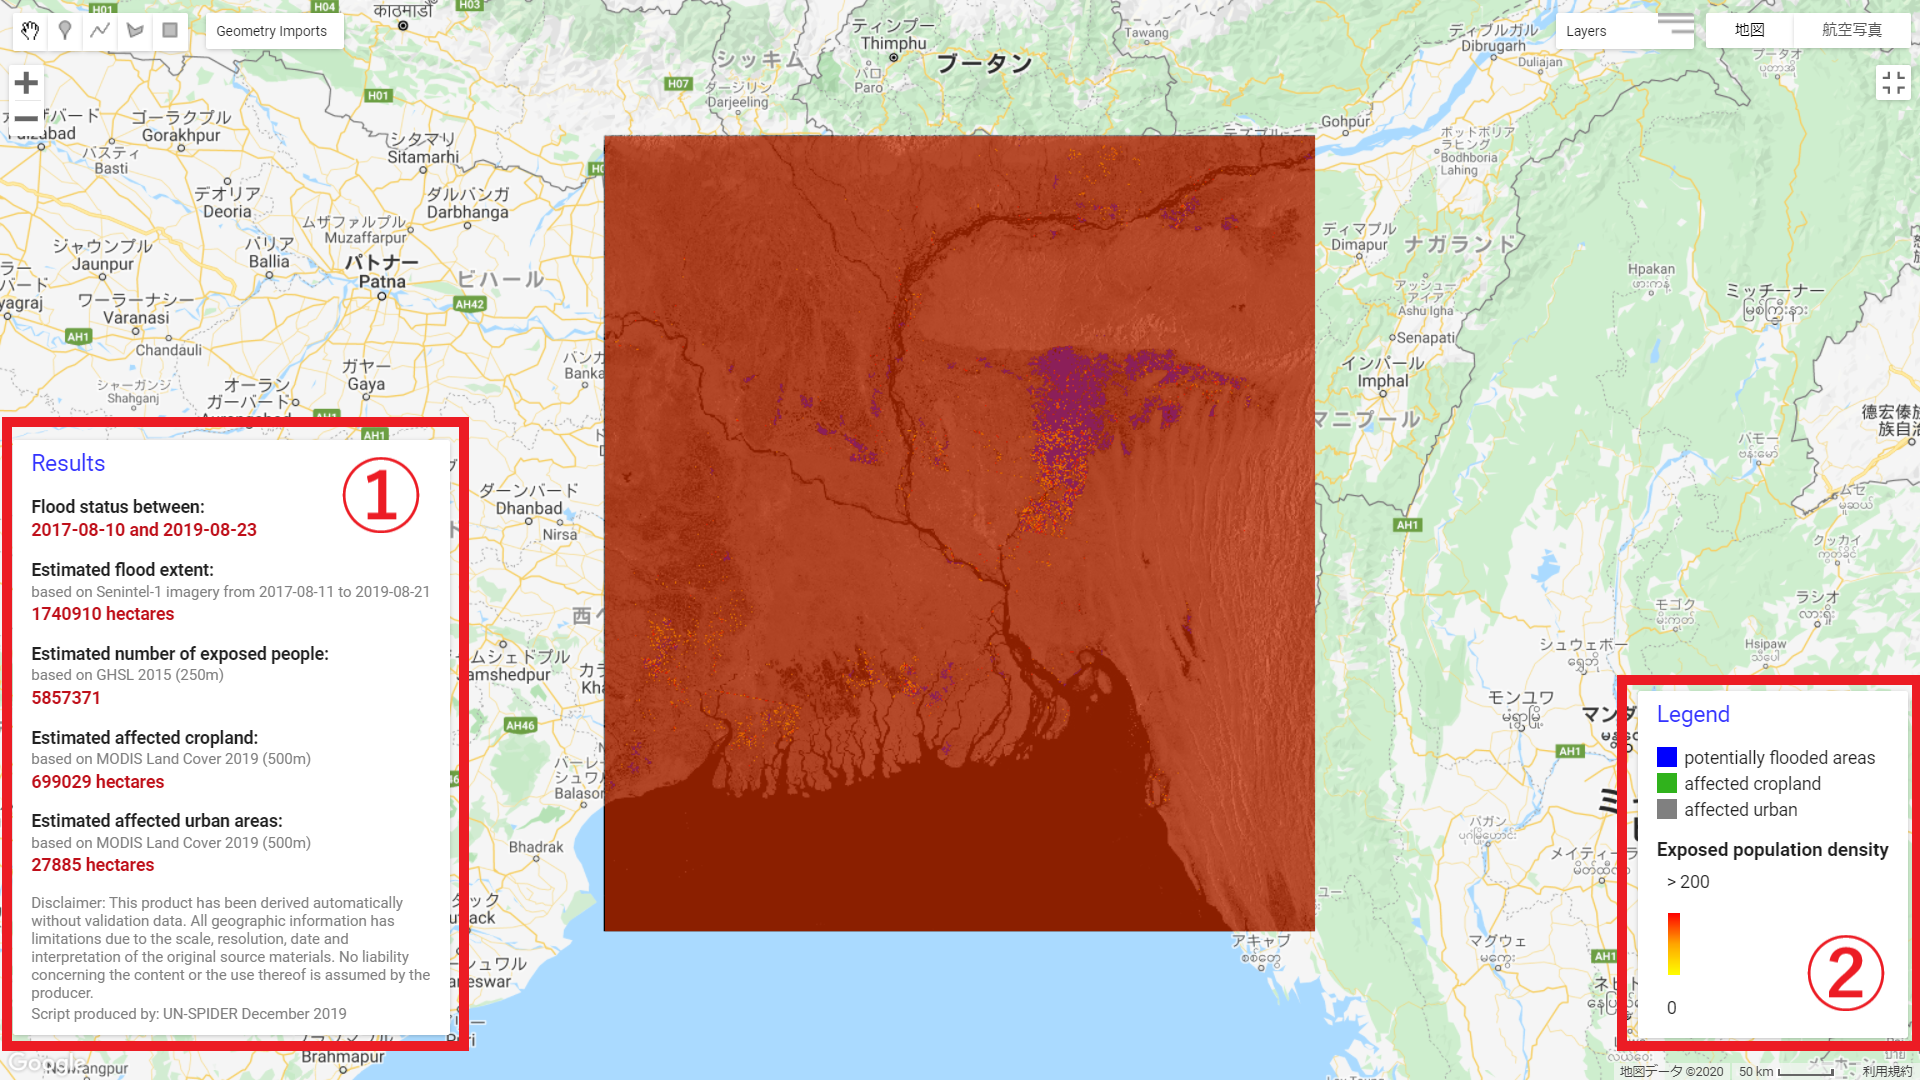
\includegraphics{images/example1.png}

\hypertarget{ux30d1ux30cdux30ebux306eux4f4dux7f6eux3092ux8a2dux5b9aux3059ux308b}{%
\subsection{パネルの位置を設定する}\label{ux30d1ux30cdux30ebux306eux4f4dux7f6eux3092ux8a2dux5b9aux3059ux308b}}

\begin{verbatim}
var legend = ui.Panel({
  style: {
    position: 'bottom-right',
    padding: '8px 15px',
  }
});
\end{verbatim}

\hypertarget{ux5857ux5206ux3051ux306eux51e1ux4f8bux3092ux4f5cux6210ux3059ux308b}{%
\subsection{塗分けの凡例を作成する}\label{ux5857ux5206ux3051ux306eux51e1ux4f8bux3092ux4f5cux6210ux3059ux308b}}

\begin{verbatim}
//凡例のタイトルを作成する
var legendTitle = ui.Label('Legend',titleTextVis);

//パネルにタイトルをつける
legend.add(legendTitle);

//凡例のスタイルを設定する
var makeRow = function(color, name) {
 
      // ラベル(カラーボックス)を作成する
      var colorBox = ui.Label({
        style: {
          backgroundColor: color,
          // Use padding to give the box height and width.
          padding: '8px',
          margin: '0 0 4px 0'
        }
      });
 
      // 説明をつける
      var description = ui.Label({
        value: name,
        style: {margin: '0 0 4px 6px'}
      });
 
      // 垂直に並べる
      return ui.Panel({
        widgets: [colorBox, description],
        layout: ui.Panel.Layout.Flow('horizontal')
      });
};

//  色
var palette =['#0000FF', '#30b21c', 'grey'];
 
// 凡例の名前を設定する
var names = ['potentially flooded areas','affected cropland','affected urban'];
 
// 色と名前を加える
for (var i = 0; i < 3; i++) {
  legend.add(makeRow(palette[i], names[i]));
  }  
\end{verbatim}

\hypertarget{exposed-population-densityux306eux51e1ux4f8bux3092ux4f5cux6210ux3059ux308b}{%
\subsection{``Exposed population density''の凡例を作成する}\label{exposed-population-densityux306eux51e1ux4f8bux3092ux4f5cux6210ux3059ux308b}}

\begin{verbatim}
var legendTitle2 = ui.Label({
value: 'Exposed population density',
style: {
fontWeight: 'bold',
fontSize: '15px',
margin: '10px 0 0 0',
padding: '0'
}
});

// パネルにタイトルをつける
legend.add(legendTitle2);

// 凡例を作成する
var lon = ee.Image.pixelLonLat().select('latitude');
var gradient = lon.multiply((populationExposedVis.max-populationExposedVis.min)/100.0).add(populationExposedVis.min);
var legendImage = gradient.visualize(populationExposedVis);
\end{verbatim}

\hypertarget{ux5730ux56f3ux4e0aux306bux51e1ux4f8bux3092ux8868ux793aux3059ux308b}{%
\section{地図上に凡例を表示する}\label{ux5730ux56f3ux4e0aux306bux51e1ux4f8bux3092ux8868ux793aux3059ux308b}}

\begin{verbatim}
// 凡例の一番上に文章を作成する?
var panel = ui.Panel({
widgets: [
ui.Label('> '.concat(populationExposedVis['max']))
],
});
 
legend.add(panel);
 
// 画像からサムネイルを作成する
var thumbnail = ui.Thumbnail({
image: legendImage,
params: {bbox:'0,0,10,100', dimensions:'10x50'},
style: {padding: '1px', position: 'bottom-center'}
});
 
// 凡例にサムネイルをつける
legend.add(thumbnail);
 
// 凡例の一番上に文章を作成する?
var panel = ui.Panel({
widgets: [
ui.Label(populationExposedVis['min'])
],
});
 
legend.add(panel);
 
// 地図上に凡例を表示させる
Map.add(legend);
\end{verbatim}

  \bibliography{book.bib,packages.bib}

\end{document}
